\documentclass[a4paper,10pt]{article}

\usepackage{graphicx}
\usepackage{url}
\usepackage{times}
\usepackage{color}
\usepackage{floatpag}

\begin{document}

\title{Ibis RMI User's Guide}

\author{http://www.cs.vu.nl/ibis}

\maketitle

\section{Introduction}

Java applications typically consist of one or more threads that
manipulate a collection of objects by invoking methods on these
objects. Figure~\ref{normal-fig} shows an example, where a single
application thread
has a reference to some interface which represents an object. The
thread and object are located in the same Java Virtual Machine (JVM),
and the thread can use normal method invocations on the interface to
manipulate the state of the object.

\begin{figure}[t]
\begin{center}
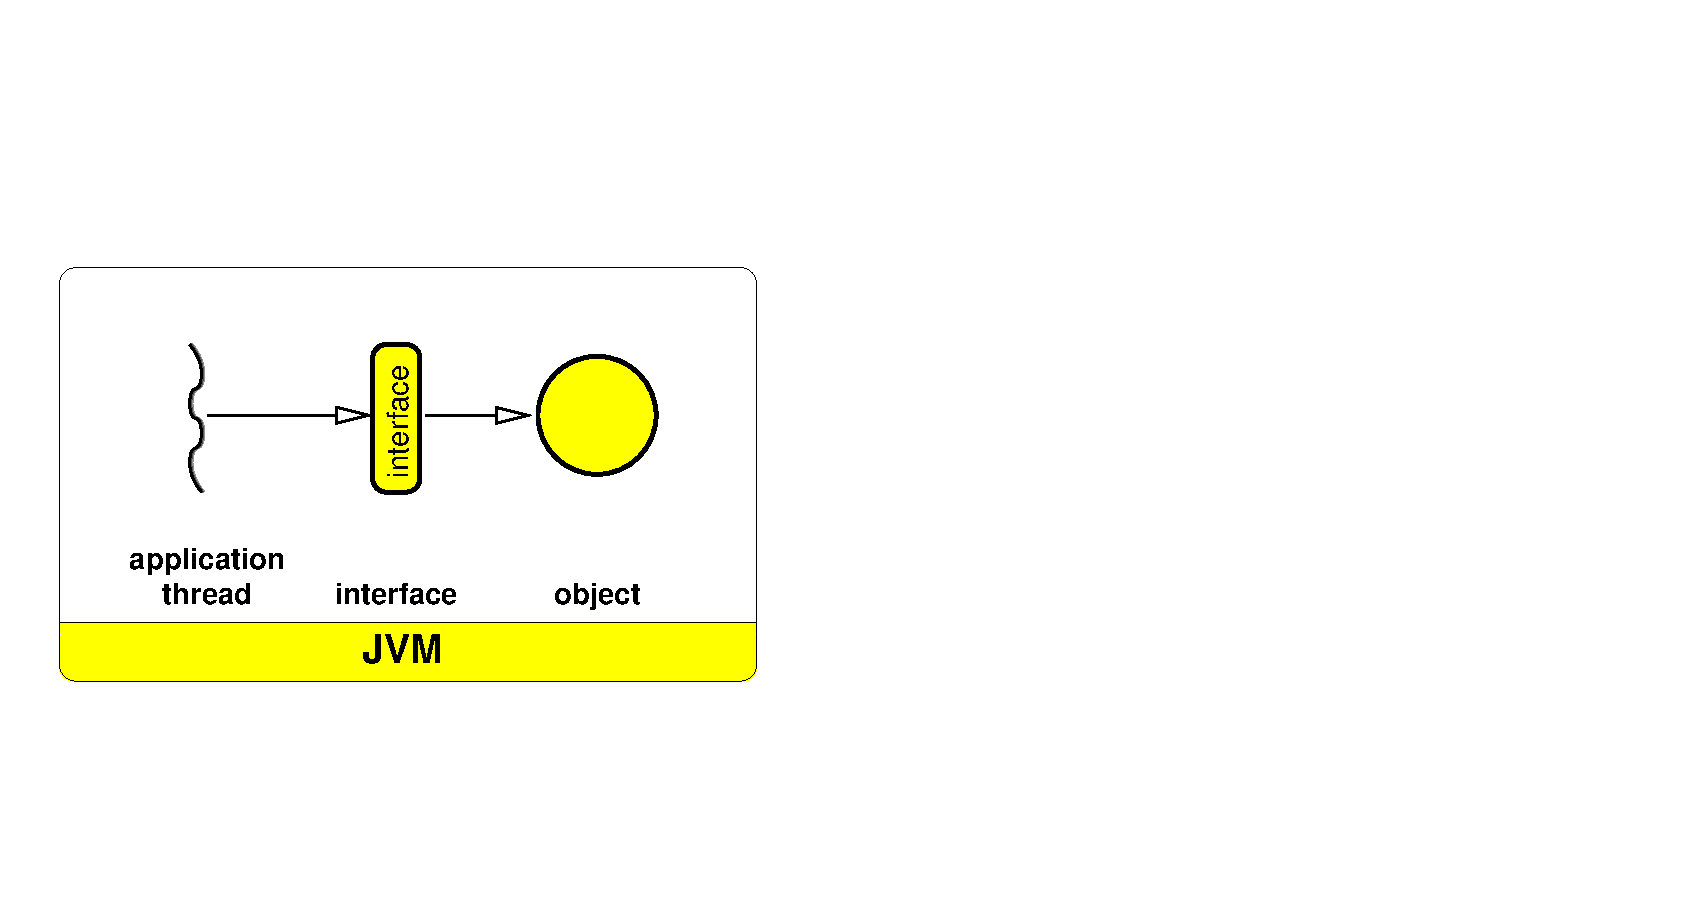
\includegraphics[width=0.7\textwidth]{normal.eps}
\end{center}
\caption{A normal invocation.}
\label{normal-fig}
\end{figure}

To turn the example of Figure~\ref{normal-fig} into a distributed RMI invocation,
some small modifications must be made to the program. The interface
must be turned into a remote interface by extending java.rmi.Remote,
and the object must be turned into a remote object by extending
java.rmi.UnicastRemoteObject. The rmic compiler, which is part of the
Java Developer Kit (JDK), can then generate the required communication
code. This code consist of two objects, a 'stub' and a 'skeleton', as
shown in Figure~\ref{rmi-fig}.

\begin{figure}[t]
\begin{center}
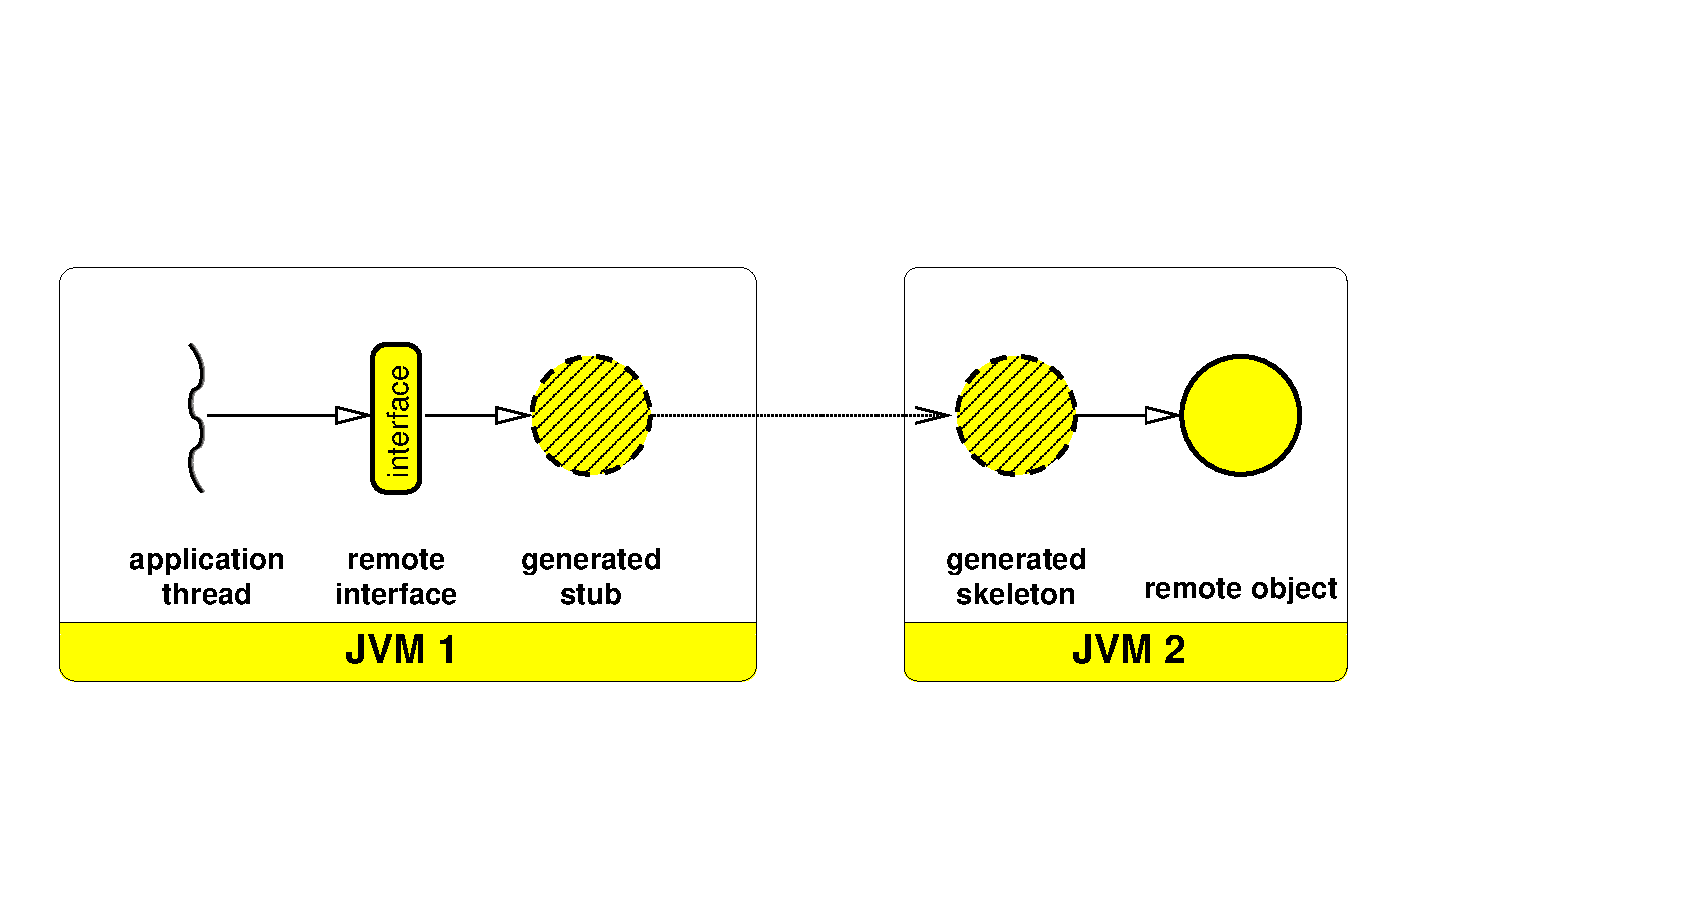
\includegraphics[width=0.7\textwidth]{rmi-abstract.eps}
\end{center}
\caption{A remote invocation with RMI.}
\label{rmi-fig}
\end{figure}

The stub object implements the application interface, and contains
code to forward any method invocations it receives to a skeleton
object on another JVM. The skeleton object contains code to receive
these invocations, and perform them on the object. It then sends the
results back to the stub, which returns them to the waiting
application thread.  Although RMI is not completely transparent, only
small modifications to the application are required. Furthermore, the
programmer does not have to write any communication code (this is
generated by rmic), making RMI easy to use. Unfortunately, the way in
which method invocations are handled in RMI is fixed. After the stub
forwards the invocation to the skeleton, it waits for a reply message
before continuing. The skeleton must therefore always send a reply
back to the stub (even if the method has no result. Furthermore, a
stub in RMI always serves as a 'remote reference' to a single object,
which can not be changed once the stub has been created.

There is very little difference between the usage of Sun RMI and Ibis
RMI. The programs are exactly the same, you only have to compile them
with Ibis \texttt{rmic} instead of the Sun \texttt{rmic}. 
This manual describes the steps required to run an RMI application
using the Ibis RMI System.

%\remark{TODO limitations/restrictions.}

Since Ibis RMI is built on top of the Ibis Portability Layer (IPL),
the Ibis RMI release contains the Ibis communication library, which contains
implementations of the IPL. Parts of this manual may look familiar for
readers that are familiar with the Ibis communication library.

\section{Compiling the TSP example}

The TSP example application for RMI is
provided with the Ibis RMI distribution, in the \texttt{examples} directory.
For convenience, the application is already compiled.

If you change the example, you will need to recompile it. This
requires the build system \texttt{ant}\footnote{\url{http://ant.apache.org}}.
Running \texttt{ant} in the examples directory compiles the example,
and rewrites the class files for use with Ibis RMI.

If, for some reason, it is not convenient to use \emph{ant} to compile
your application, or you have only class files or jar files available
for parts of your application, it is also possible to first compile
your application to class files or jar files, and then process those
using the \emph{rmic} script. This script can be found in the Ibis RMI
bin directory. It takes either directories, class files, or jar files
as parameter, and processes those, possibly rewriting them. In case
of a directory, all class files and jar files in that directory or
its subdirectories are processed.  The command sequence

\begin{verbatim}
$ cd $RMI_HOME/examples
$ mkdir tmp
$ javac -d tmp -g \
     -classpath ../external/ipl/ibis-poolinfo-2.1.1.jar \
     src/tsp/*.java src/shared/*.java
$ ../bin/rmic -cp tmp tmp
$ mkdir lib
$ ( cd tmp ; jar c . ) > lib/rmi-examples.jar
$ rm -rf tmp
\end{verbatim}

creates a \texttt{lib} directory and stores the resulting class files there,
in a jar-file called \texttt{rmi-examples.jar}.
The \texttt{RMI\_HOME} environment variable must be set to the location of
the Ibis RMI installation.

\section{An Ibis RMI run}

Before discussing
the running of an Ibis RMI application, we will discuss services that are
needed by the Ibis communication library.

\subsection{The pool}

A central concept in Ibis is the \emph{Pool}. A pool consists of one or
more Ibis instances, usually running on different machines. Each pool is
generally made up of Ibises running a single distributed application.
Ibises in a pool can communicate with each other, and, using the
registry mechanism present in Ibis, can search for other Ibises in the
same pool, get notified of Ibises joining the pool, etc. To
coordinate Ibis pools a so-called \emph{Ibis server} is used.

\subsection{The Ibis Server}

The Ibis server is the Swiss-army-knife server of the Ibis project.
Services can be dynamically added to the server. By default, the Ibis
communication library comes with a registry service. This registry
service manages pools, possibly multiple pools at the same time.

In addition to the registry service, the server also allows
Ibises to route traffic over the server if no direct connection is
possible between two instances due to firewalls or NAT boxes. This is
done using the Smartsockets library of the Ibis project.

The Ibis server is started with the \texttt{rmi-server} script which is
located in the \texttt{bin} directory of the Ibis RMI distribution.  Before
starting an Ibis RMI application, an Ibis server needs to be running on a
machine that is accessible from all nodes participating in the Ibis RMI run.
The server listens to a TCP port. The port number can be specified using
the \texttt{--port} command line option to the \texttt{rmi-server}
script.  For a complete list of all options, use the \texttt{--help}
option of the script. One useful option is the  \texttt{--events}
option, which makes the registry print out events.

\subsubsection{Hubs}
\label{hubs}

The Ibis server is a single point which needs to be reachable from every
Ibis instance. Since sometimes this is not possible due to firewalls,
additional \emph{hubs} can be started to route traffic, creating a
routing infrastructure for the Ibis RMI instances. These hubs can be started
by using rmi-server script with the \texttt{--hub-only} option. In
addition, each hub needs to know the location of as many of the other
hubs as possible. This information can be provided by using the
\texttt{--hub-addresses} option. See the \texttt{--help} option of the
rmi-server script for more information.

\subsection{Running the example: preliminaries}

When the Ibis server is running, the Ibis RMI application itself can be
started.  There are a number of requirements that need to be met before
Ibis (and thus Ibis RMI) can be started correctly.
In this section we will discuss these in detail.

Several of the steps below require the usage of \emph{system properties}.
System properties can be set in Java using the \texttt{-D} option of the
\texttt{java} command. Be sure to use appropriate quoting for your
command interpreter.

As an alternative to using system properties, it is also possible to use
a java properties file
\footnote{\url{http://java.sun.com/j2se/1.5.0/docs/api/java/util/Properties.html}}.
A properties file is a file containing one property per line, usually of
the format \texttt{property = value}. Properties of Ibis can be set in
such a file as if they were set on the command line directly.

Ibis and Ibis RMI will look for a file named \texttt{ibis.properties} in the
current working directory, on the class path, and at a location specified
with the \texttt{ibis.properties.file} system property.

\subsubsection{Add jar files to the classpath}

The Ibis RMI implementation is provided in a single jar file: rmi.jar,
appended with the version of Ibis RMI, for instance \texttt{rmi-2.1.jar}.
Ibis RMI interfaces to Ibis using the Ibis Portability Layer, or
\emph{IPL}. Both Ibis RMI and the IPL depend on various other libraries.
All jar files in \$RMI\_HOME/lib need to be on the classpath.

\subsubsection{Configure Log4j}

Ibis and Ibis RMI use the Log4J library of the Apache project to print debugging
information, warnings, and error messages. This library must be
initialized. A configuration file can be specified using the
\texttt{log4j.configuration} system property. For example, to use a file
named \texttt{log4j.properties} in the current directory, use the
following command line option:
\texttt{-Dlog4j.configuration=file:log4j.properties}. For more info,
see the log4j website \footnote{\url{http://logging.apache.org/log4j}}.

\subsubsection{Set the location of the server and hubs}

To communicate with the registry service, each Ibis instance needs the address
of the Ibis server. This address must be specified by using the
\texttt{ibis.server.address} system property. The full address needed is
printed on start up of the Ibis server.

For convenience, it is also possible to only provide an address, port number
pair, e.g. \texttt{machine.domain.com:5435} or even simply a host, e.g.
\texttt{localhost}. In this case, the default port number (8888) is implied.
The port number provided must match the one given to the Ibis server
with the \texttt{--port} option.

When additional hubs are started (see Section \ref{hubs}), their locations
must be provided to the Ibis instances. This can be done using
the \texttt{ibis.hub.addresses} property. Ibis expects a comma-separated
list of addresses of hubs. Ibis will use the first reachable hub on the
list. The address of the Ibis server is appended to this list
automatically. Thus, by default, the Ibis server itself is used as the
hub.

\subsubsection{Set the name and size of the pool}

Each Ibis instance belongs to a pool. The name of this pool must be provided
using the \texttt{ibis.pool.name} property. With the help of the Ibis server,
this name is then used to locate other Ibis instances which belong to the
same pool. Since the Ibis server can service multiple pools simultaneously,
each pool must have a unique name.

It is possible for pools to have a fixed size. In these so-called \emph{closed
world} pools, the number of Ibises in the pool is also needed to function
correctly. This size must be set using the \texttt{ibis.pool.size} property.
This property is normally not needed. When it is needed, but not provided, Ibis
will print an error. 

\subsubsection{The rmi-run script}

To simplify running an Ibis RMI application, a \texttt{rmi-run} script is
provided with the distribution. This script can be
used as follows

\begin{center}
\texttt{rmi-run} \emph{java-flags class parameters}
\end{center}

The script performs the first two steps needed to run an Ibis RMI application.
It adds all required jar files
to the class path, and configures log4j.
It then runs \texttt{java} with any
command line options given to it. Therefore, any additional options for
Java, the main class and any application parameters must be provided as
if \texttt{java} was called directly.

The \texttt{rmi-run} script needs the location of the Ibis RMI
distribution. This must be provided using the RMI\_HOME environment
variable.

\subsection{Running the example on Unix-like systems}

This section is specific for Unix-like systems. In particular, the
commands presented are for a Bourne shell or bash.

We will now run the example. All code below assumes the RMI\_HOME
environment variable is set to the location of the Ibis RMI distribution.

First, we will need an Ibis server. Start a shell and
run the \texttt{rmi-server} script:
\noindent
{\small
\begin{verbatim}
$ $RMI_HOME/bin/rmi-server --events
\end{verbatim}
}
\noindent

By providing the \texttt{--events} option the server
prints information on when Ibis instances join and leave the pool.

Next, we will start the application two times. One instance will act as both
an "RMI server" and an "RMI client", the other one will just be an "RMI client".
Ibis RMI will determine who is who automatically. Therefore we can using the
same command line for both instances.
Run the following command in two different shells:

\noindent
{\small
\begin{verbatim}
$ CLASSPATH=$RMI_HOME/examples/lib/rmi-examples.jar \
    $RMI_HOME/bin/rmi-run \
    -Dibis.server.address=localhost \
    -Dibis.pool.size=2 -Dibis.pool.name=test \
    tsp.Main $RMI_HOME/examples/src/tsp/table_15.1
\end{verbatim}
}
\noindent

This sets the CLASSPATH environment variable to the jar file of the
application, and calls rmi-run. You should now have two running
instances of your application. One of them should print:

\noindent
{\small
\begin{verbatim}
I am 130.37.193.40
Getting registry on 130.37.193.40
Got registry on 130.37.193.40
Distance table read
2184 Jobs generated
Minimum route = 3162
Calculation Time = 13996 ms; Parallel time 13708 ms
TSP-RMI took 13.996 seconds
\end{verbatim}
}
\noindent

or something similar.

As said, the rmi-run script is only provided for convenience. To run
the application without rmi-run, the command below can be used.
Note that this only works with Java 6. For Java 1.5, you need to
explicitly add all jar files in \$RMI\_HOME/lib to the classpath.

\noindent
{\small
\begin{verbatim}
$ java \
    -cp \
    $RMI_HOME/lib/'*':$RMI_HOME/examples/lib/rmi-examples.jar \
    -Dibis.server.address=localhost \
    -Dibis.pool.name=test -Dibis.pool.size=2 \
    -Dlog4j.configuration=file:$RMI_HOME/log4j.properties \
    tsp.Main $RMI_HOME/examples/src/tsp/table_15.1
\end{verbatim}
}
\noindent

\subsection{Running the example on Windows systems}

We will now run the example on a Windows XP system.
All code below assumes the RMI\_HOME
environment variable is set to the location of the Ibis RMI distribution.

First, we will need an Ibis server. Start a command prompt window and
run the \texttt{rmi-server} script:
\noindent
{\small
\begin{verbatim}
C:\DOCUME~1\Temp> "%RMI_HOME%"\bin\rmi-server --events
\end{verbatim}
}
\noindent

Note the quoting, which is needed when RMI\_HOME contains spaces.

By providing the \texttt{--events} option the server
prints information on when Ibis instances join and leave the pool.

Next, we will start the application two times. One instance will act as both an
"RMI server" and an "RMI client", the other one will be an "RMI client".
Ibis RMI will determine who is who automatically. Therefore we can using the
same command line for both server and client.
Run the following command in two different shells:

\noindent
{\small
\begin{verbatim}
C:\DOCUME~1\Temp> set CLASSPATH=%RMI_HOME%\examples\lib\rmi-examples.jar
C:\DOCUME~1\Temp> "%RMI_HOME%"\bin\rmi-run
    "-Dibis.server.address=localhost"
    "-Dibis.pool.size=2" "-Dibis.pool.name=test"
    tsp.Main "%RMI_HOME%"\examples\src\tsp\table_15.1
\end{verbatim}
}
\noindent

This sets the CLASSPATH environment variable to the jar file of the
application, and calls rmi-run. You should now have two running
instances of your application. One of them should print:

\noindent
{\small
\begin{verbatim}
I am 130.37.193.40
Getting registry on 130.37.193.40
Got registry on 130.37.193.40
Distance table read
2184 Jobs generated
Minimum route = 3162
Calculation Time = 13996 ms; Parallel time 13708 ms
TSP-RMI took 13.996 seconds
\end{verbatim}
}
\noindent

or something similar.

As said, the rmi-run script is only provided for convenience. To run
the application without rmi-run, the command below can be used.
Note that this only works with Java 6. For Java 1.5, you need to
explicitly add all jar files in \%RMI\_HOME\%$\backslash$lib to the classpath.

\noindent
{\small
\begin{verbatim}
C:\DOCUME~1\Temp> java
    -cp "%RMI_HOME%\lib\*";"%RMI_HOME%"\examples\lib\rmi-examples.jar
    -Dibis.server.address=localhost
    -Dibis.pool.name=test -Dibis.pool.size=2
    -Dlog4j.configuration=file:"%RMI_HOME%"\log4j.properties
    tsp.Main "%RMI_HOME%"\examples\src\tsp\table_15.1
\end{verbatim}
}
\noindent

\section{Further Reading}

The Ibis web page \url{http://www.cs.vu.nl/ibis} lists all
the documentation and software available for Ibis, including papers, and
slides of presentations.

\end{document}

